\documentclass{beamer}
\usepackage{amsmath}
\usepackage[english]{babel} %set language; note: after changing this, you need to delete all auxiliary files to recompile
\usepackage[utf8]{inputenc} %define file encoding; latin1 is the other often used option
\usepackage{csquotes} % provides context sensitive quotation facilities
\usepackage{graphicx} %allows for inserting figures
\usepackage{booktabs} % for table formatting without vertical lines
\usepackage{textcomp} % allow for example using the Euro sign with \texteuro
\usepackage{stackengine}
\usepackage{wasysym}
\usepackage{tikzsymbols}
\usepackage{textcomp}
\usepackage{xcolor}
\usepackage[dvipsnames]{xcolor}
\usepackage{colortbl}
\usepackage{adjustbox}
\usepackage{tikz}
\usetikzlibrary{arrows.meta, calc, decorations.pathreplacing}


\usepackage{amssymb}
\usepackage{multirow}

% Colores
\definecolor{rojo}{RGB}{221, 36, 36}
\definecolor{celeste}{RGB}{173, 216, 230}

\newcommand{\up}{\textcolor{blue}{\Large$\uparrow$}}
\newcommand{\down}{\textcolor{red}{\Large$\downarrow$}}
\newcommand{\question}{\textcolor{red}{\Large\textbf{?}}}


% ELIMINAR COMANDOS DE NAVEGACION%%%%%%%%%%%
\setbeamertemplate{navigation symbols}

%\newcommand{\bubblethis}[2]{
 %       \tikz[remember picture,baseline]{\node[anchor=base,inner sep=0,outer sep=0]%
 %       (#1) {\underline{#1}};\node[overlay,cloud callout,callout relative pointer={(0.2cm,-0.7cm)},%
 %       aspect=2.5,fill=yellow!90] at ($(#1.north)+(-0.5cm,1.6cm)$) {#2};}%
 %   }%
%\tikzset{face/.style={shape=circle,minimum size=4ex,shading=radial,outer sep=0pt,
 %       inner color=white!50!yellow,outer color= yellow!70!orange}}

%% Some commands to make the code easier
\newcommand{\emoticon}[1][]{%
  \node[face,#1] (emoticon) {};
  %% The eyes are fixed.
  \draw[fill=white] (-1ex,0ex) ..controls (-0.5ex,0.2ex)and(0.5ex,0.2ex)..
        (1ex,0.0ex) ..controls ( 1.5ex,1.5ex)and( 0.2ex,1.7ex)..
        (0ex,0.4ex) ..controls (-0.2ex,1.7ex)and(-1.5ex,1.5ex)..
        (-1ex,0ex)--cycle;}
\newcommand{\pupils}{
  %% standard pupils
  \fill[shift={(0.5ex,0.5ex)},rotate=80] 
       (0,0) ellipse (0.3ex and 0.15ex);
  \fill[shift={(-0.5ex,0.5ex)},rotate=100] 
       (0,0) ellipse (0.3ex and 0.15ex);}

\newcommand{\emoticonname}[1]{
  \node[below=1ex of emoticon,font=\footnotesize,
        minimum width=4cm]{#1};}
\usepackage{scalerel}
\usetikzlibrary{positioning}
\usepackage{xcolor,amssymb}
\newcommand\dangersignb[1][2ex]{%
  \scaleto{\stackengine{0.3pt}{\scalebox{1.1}[.9]{%
  \color{red}$\blacktriangle$}}{\tiny\bfseries !}{O}{c}{F}{F}{L}}{#1}%
}
\newcommand\dangersignw[1][2ex]{%
  \scaleto{\stackengine{0.3pt}{\scalebox{1.1}[.9]{%
  \color{red}$\blacktriangle$}}{\color{white}\tiny\bfseries !}{O}{c}{F}{F}{L}}{#1}%
}
\usepackage{fontawesome} % Social Icons
\usepackage{epstopdf} % allow embedding eps-figures
\usepackage{tikz} % allows drawing figures
\usepackage{amsmath,amssymb,amsthm} %advanced math facilities
\usepackage{lmodern} %uses font that support italic and bold at the same time
\usepackage{hyperref}
\usepackage{tikz}
\hypersetup{
    colorlinks=true,
    linkcolor=blue,
    filecolor=magenta,      
    urlcolor=blue,
}
\usepackage{tcolorbox}
%add citation management using BibLaTeX
\usepackage[citestyle=authoryear-comp, %define style for citations
    bibstyle=authoryear-comp, %define style for bibliography
    maxbibnames=10, %maximum number of authors displayed in bibliography
    minbibnames=1, %minimum number of authors displayed in bibliography
    maxcitenames=3, %maximum number of authors displayed in citations before using et al.
    minnames=1, %maximum number of authors displayed in citations before using et al.
    datezeros=false, % do not print dates with leading zeros
    date=long, %use long formats for dates
    isbn=false,% show no ISBNs in bibliography (applies only if not a mandatory field)
    url=false,% show no urls in bibliography (applies only if not a mandatory field)
    doi=false, % show no dois in bibliography (applies only if not a mandatory field)
    eprint=false, %show no eprint-field in bibliography (applies only if not a mandatory field)
    backend=biber %use biber as the backend; backend=bibtex is less powerful, but easier to install
    ]{biblatex}
\addbibresource{../mybibfile.bib} %define bib-file located one folder higher


\usefonttheme[onlymath]{serif} %set math font to serif ones

\definecolor{beamerblue}{rgb}{0.2,0.2,0.7} %define beamerblue color for later use

%%% defines highlight command to set text blue
\newcommand{\highlight}[1]{{\color{blue}{#1}}}


%%%%%%% commands defining backup slides so that frame numbering is correct

\newcommand{\backupbegin}{
   \newcounter{framenumberappendix}
   \setcounter{framenumberappendix}{\value{framenumber}}
}
\newcommand{\backupend}{
   \addtocounter{framenumberappendix}{-\value{framenumber}}
   \addtocounter{framenumber}{\value{framenumberappendix}}
}

%%%% end of defining backup slides

%Specify figure caption, see also http://tex.stackexchange.com/questions/155738/caption-package-not-working-with-beamer
\setbeamertemplate{caption}{\insertcaption} %redefines caption to remove label "Figure".
%\setbeamerfont{caption}{size=\scriptsize,shape=\itshape,series=\bfseries} %sets figure  caption bold and italic and makes it smaller


\usetheme{Boadilla}

%set options of hyperref package
\hypersetup{
    bookmarksnumbered=true, %put section numbers in bookmarks
    naturalnames=true, %use LATEX-computed names for links
    citebordercolor={1 1 1}, %color of border around cites, here: white, i.e. invisible
    linkbordercolor={1 1 1}, %color of border around links, here: white, i.e. invisible
    colorlinks=true, %color links
    anchorcolor=black, %set color of anchors
    linkcolor=beamerblue, %set link color to beamer blue
    citecolor=blue, %set cite color to beamer blue
    pdfpagemode=UseThumbs, %set default mode of PDF display
    breaklinks=true, %break long links
    pdfstartpage=1 %start at first page
    }

\newtcolorbox{boxA}{
    fontupper = \bf,
    boxrule = 1.5pt,
    colframe = black % frame color
}
\newtcolorbox{boxB}{
    boxrule = 1.5pt,
    colframe = blue!70!black,, % frame color
    colback = blue!7!white,
}

% --------------------
% Overall information
% --------------------
\title[Economía I]{Economía I \vspace{3mm}
\\ Magistral 10 \vspace{3mm} \\ Equilibrio de mercado}
\date{}
\author[Victoria Rosino]{Victoria Rosino}
\vspace{0.3cm}
\institute[]{Universidad de San Andrés} 

\begin{document}

\begin{frame}
\vspace{0.3cm}
\titlepage
\centering
\vspace{-0.9cm}
\includegraphics[scale=0.3]{Slides Principios de Economia/Figures/udesa_logo.jpg} 
\end{frame}


\begin{frame}
\frametitle{Motivación: El precio del petróleo}
\centering
\includegraphics[scale=1]{Slides Principios de Economia/Figures/Magistral_10/M10.1.png}
\end{frame} 

\begin{frame}
\frametitle{Al precio lo determinan la demanda y la oferta}
\begin{itemize}
    \item Por un lado, tenemos la curva de demanda
    \begin{itemize}
        \item Muestra la cantidad total que los consumidores están dispuestos a comprar a cualquier precio dado.
        \item Representa la máxima disposición a pagar en dinero por los productos que compran.
        \item Detrás de la demanda sabemos que está la utilidad marginal (\textit{decreciente}) que los consumidores reciben de cada unidad adicional.
    \end{itemize}
    \vspace{2mm}
    \item Por otro lado, tenemos la curva de oferta
    \begin{itemize}
        \item Muestra la cantidad total que las empresas producirían a cualquier precio dado.
        \item Representa la mínima disposición a aceptar en dinero por los productos que venden, es decir, refleja los distintos precios de reserva de estos vendedores.
        \item Detrás de la oferta sabemos que está el costo marginal (\textit{creciente}) que las empresas tienen al producir cada unidad adicional.
        \end{itemize}
\end{itemize}
\end{frame}

\begin{frame}
\frametitle{Las curvas se cruzan en un punto}
    \begin{figure}[H]
    \begin{center}
        \begin{tikzpicture}[scale=1.1]
        \draw[thick,->] (0,0) -- (6,0) node[below] {$Q$};
        \draw[thick,->] (0,0) -- (0,6) node[left] {$P$};

        %Demanda
        \draw [thick, Blue] (0,5) -- (5,0);
        \node [right, Blue] at (4.8,0.4) {$D$};
        %Oferta
        \draw [thick, RubineRed] (0,0) -- (5,5);
        \node [right, RubineRed] at (5,5) {$O$};

        % Punto E
        \draw[dashed, gray] (2.5,0) -- (2.5,2.5);
        \draw[dashed, gray] (0,2.5) -- (2.5,2.5);
        \fill (2.5,2.5) circle (3pt);
        \node [above] at (2.5,2.6) {$E$};
        \node[below] at (2.5,0) {$Q^*$};
        \node[left] at (0,2.5) {$P^*$};
        
        \end{tikzpicture}
    \end{center}
    \end{figure}
\end{frame}

\begin{frame}{Equilibrio}
    \begin{itemize}
        \item En el precio de equilibrio se igualan las cantidades ofrecidas con las cantidades demandadas.
        \item Si el precio es superior al de equilibrio ($P > P^*$), hay un exceso de oferta. Si esto pasa, los productores decidirán disminuir sus precios, aumentando la cantidad demandadas y disminuyendo las cantidades ofrecidas.
        \item Si el precio es inferior al de equilibrio ($P < P^*$), hay un exceso de demanda. Hay escasez en el mercado. Los productores observan esta situación, aumentan los precios, disminuyendo la cantidad demandada y aumentando la cantidad ofrecida.
        \item En ambos casos lo que tiene que quedar claro es que nos movemos \textbf{a lo largo de las curvas} de oferta y demanda. No se desplazan las curvas cuando lo que se mueve es el precio\dots
    \end{itemize}
\end{frame}

\begin{frame}
\frametitle{Exceso de oferta}
\begin{center}
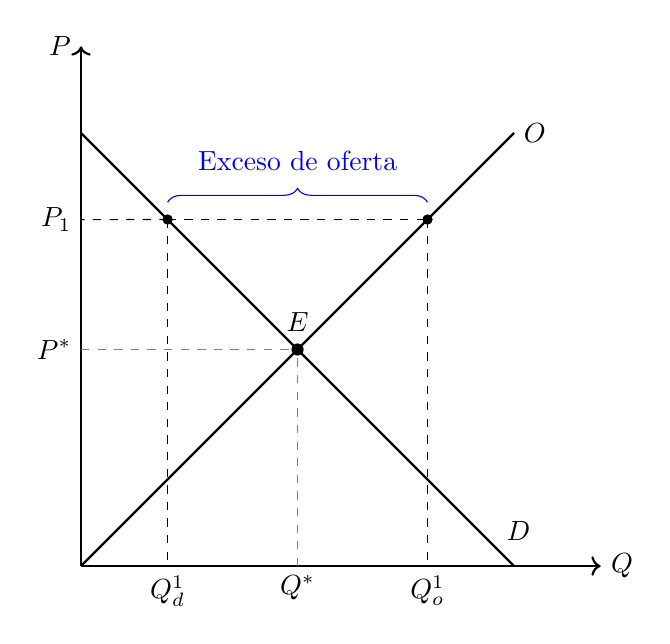
\begin{tikzpicture}[scale=1.1]

% Ejes
\draw[thick, ->] (0,0) -- (6,0) node[right] {$Q$};
\draw[thick, ->] (0,0) -- (0,6) node[left] {$P$};

% Curvas de oferta y demanda
\draw [thick] (0,5) -- (5,0);
\node [right] at (4.8,0.4) {$D$};
\draw [thick] (0,0) -- (5,5);
\node [right] at (5,5) {$O$};

% Precio de equilibrio y líneas punteadas
\draw[dashed, gray] (2.5,0) -- (2.5,2.5);
\draw[dashed, gray] (0,2.5) -- (2.5,2.5);
\fill (2.5,2.5) circle (2pt);
\node [above] at (2.5,2.6) {$E$};
\node[below] at (2.5,0) {$Q^*$};
\node[left] at (0,2.5) {$P^*$};

% Precio P1 más alto
\coordinate (P1L) at (1,4);
\coordinate (P1R) at (4,4);
\filldraw[black] (P1L) circle (1.5pt);
\filldraw[black] (P1R) circle (1.5pt);
\draw[dashed] (P1L) -- (P1R);
\draw[dashed] (P1L) -- (P1L |- 0,0) node[below] {$Q^1_d$};
\draw[dashed] (P1R) -- (P1R |- 0,0) node[below] {$Q^1_o$};
\draw[dashed] (P1L) -- (0,4) node[left] {$P_1$};

% Exceso de oferta
\draw[decorate,decoration={brace, amplitude=5pt},draw=Blue,
text=Blue] (1,4.2) -- (4,4.2) node[midway, above=8pt] {Exceso de oferta};

\end{tikzpicture}
\end{center}
\end{frame}

\begin{frame}
\frametitle{Exceso de demanda}
\begin{center}
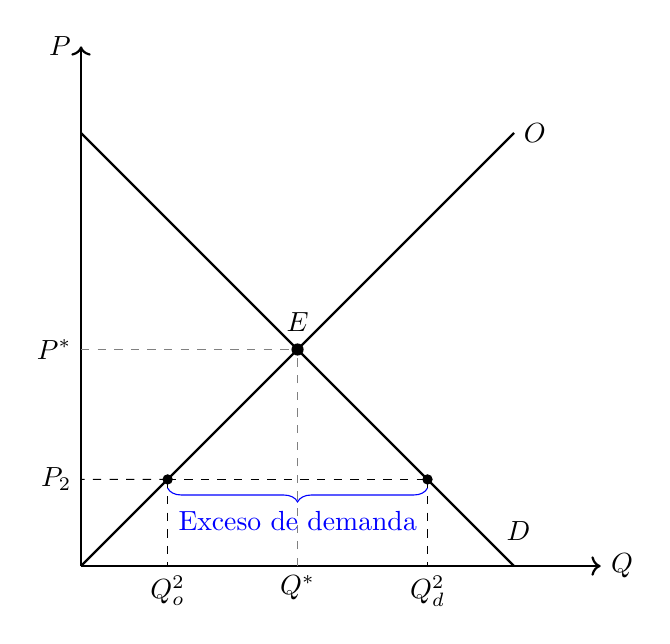
\begin{tikzpicture}[scale=1.1]

% Ejes
\draw[thick, ->] (0,0) -- (6,0) node[right] {$Q$};
\draw[thick, ->] (0,0) -- (0,6) node[left] {$P$};

% Curvas de oferta y demanda
\draw [thick] (0,5) -- (5,0);
\node [right] at (4.8,0.4) {$D$};
\draw [thick] (0,0) -- (5,5);
\node [right] at (5,5) {$O$};

% Precio de equilibrio y líneas punteadas
\draw[dashed, gray] (2.5,0) -- (2.5,2.5);
\draw[dashed, gray] (0,2.5) -- (2.5,2.5);
\fill (2.5,2.5) circle (2pt);
\node [above] at (2.5,2.6) {$E$};
\node[below] at (2.5,0) {$Q^*$};
\node[left] at (0,2.5) {$P^*$};

% Precio P1 más alto
\coordinate (P2L) at (1,1);
\coordinate (P2R) at (4,1);
\filldraw[black] (P2L) circle (1.5pt);
\filldraw[black] (P2R) circle (1.5pt);
\draw[dashed] (P2L) -- (P2R);
\draw[dashed] (P2L) -- (P2L |- 0,0) node[below] {$Q^2_o$};
\draw[dashed] (P2R) -- (P2R |- 0,0) node[below] {$Q^2_d$};
\draw[dashed] (P2L) -- (0,1) node[left] {$P_2$};

% Exceso de demanda
\draw[decorate,decoration={brace, mirror, amplitude=5pt},draw=Blue,
text=Blue] (1,0.9) -- (4,0.9) node[midway, below=5pt] {Exceso de demanda};

\end{tikzpicture}
\end{center}
\end{frame}

\begin{frame}
\frametitle{Cambios en los factores subyacentes}
\begin{itemize}
    \item Recordemos que detrás de las curvas, existen factores que afectan a la oferta y a la demanda, desplazándolas.
    \item Veremos algunos ejemplos:
    \begin{enumerate}
        \item Aumento en el precio de un bien sustituto.
        \item Aumento en el costo de producir.
        \item Caída en los ingresos y avance tecnológico.
    \end{enumerate}
    \item Estos ejemplos nos permiten ver cómo se mueven las curvas de oferta y demanda y cómo se llega a un nuevo equilibrio.
    \item A cada ejemplo podemos replicarlo con cualquier otro caso, la idea solo es ver que sucede en el equilibrio.
\end{itemize}
\end{frame}

\begin{frame}
\frametitle{Ejemplo 1. Aumento en el precio de un bien sustituto}
    \begin{figure}[H]
    \begin{center}
        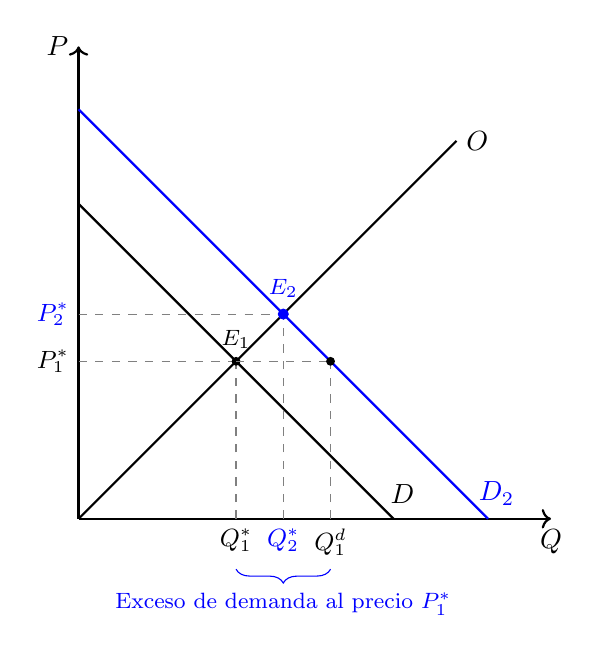
\begin{tikzpicture}[scale=0.8]
        \draw[thick,->] (0,0) -- (7.5,0) node[below] {$Q$};
        \draw[thick,->] (0,0) -- (0,7.5) node[left] {$P$};

        %Demanda
        \draw [thick] (0,5) -- (5,0);
        \node [right] at (4.8,0.4) {$D$};
        %Oferta
        \draw [thick] (0,0) -- (6,6);
        \node [right] at (6,6) {$O$};

        % Punto E
        \draw[dashed, gray] (2.5,0) -- (2.5,2.5);
        \draw[dashed, gray] (0,2.5) -- (2.5,2.5);
        \fill (2.5,2.5) circle (2pt);
        \node [above] at (2.5,2.55) {\footnotesize $E_1$};
        \node[below] at (2.5,0) {\small $Q_{1}^{*}$};
        \node[left] at (0,2.5) {\small $P_{1}^{*}$};

        % Cambios de demanda
        \draw [thick, blue] (0,6.5) -- (6.5,0);
        \node [right, blue] at (6.2,0.4) {$D_2$};

        \draw[dashed, gray] (3.25,0) -- (3.25,3.25);
        \draw[dashed, gray] (0,3.25) -- (3.25,3.25);
        \fill[blue] (3.25,3.25) circle (2.5pt);
        \node [above, blue] at (3.25,3.35) {\footnotesize $E_2$};
        \node[below, blue] at (3.25,0) {\small $Q_{2}^{*}$};
        \node[left, blue] at (0,3.25) {\small $P_{2}^{*}$};

        \draw[dashed, gray] (2.5,2.5) -- (4,2.5);
        \draw[dashed, gray] (4,0) -- (4,2.5);
        \fill (4,2.5) circle (2pt);
        \node[below] at (4,0) {\small $Q_{1}^{d}$};

        % Exceso de demanda
        \draw[decorate,decoration={brace, mirror, amplitude=5pt},draw=blue, text=blue] (2.5,-0.8) -- (4,-0.8) node[midway, below=5pt] {\footnotesize Exceso de demanda al precio $P_{1}^{*}$};

        \end{tikzpicture}
    \end{center}
    \end{figure}
\end{frame}

\begin{frame}
\frametitle{Ejemplo 2. Aumenta el costo de producir el bien}
    \begin{figure}[H]
    \begin{center}
        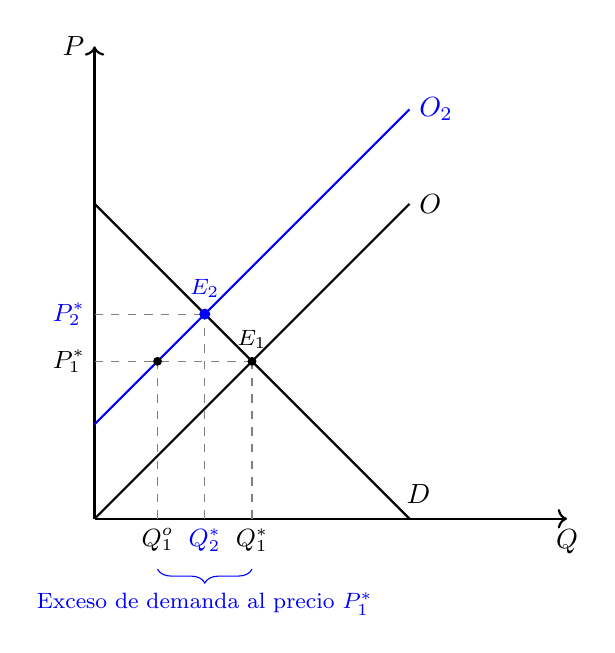
\begin{tikzpicture}[scale=0.8]
        \draw[thick,->] (0,0) -- (7.5,0) node[below] {$Q$};
        \draw[thick,->] (0,0) -- (0,7.5) node[left] {$P$};

        %Demanda
        \draw [thick] (0,5) -- (5,0);
        \node [right] at (4.8,0.4) {$D$};
        %Oferta
        \draw [thick] (0,0) -- (5,5);
        \node [right] at (5,5) {$O$};

        % Punto E
        \draw[dashed, gray] (2.5,0) -- (2.5,2.5);
        \draw[dashed, gray] (0,2.5) -- (2.5,2.5);
        \fill (2.5,2.5) circle (2pt);
        \node [above] at (2.5,2.55) {\footnotesize $E_1$};
        \node[below] at (2.5,0) {\small $Q_{1}^{*}$};
        \node[left] at (0,2.5) {\small $P_{1}^{*}$};

        % Cambios de ofera
        \draw [thick, blue] (0,1.5) -- (5,6.5);
        \node [right, blue] at (5,6.5) {$O_2$};

        \draw[dashed, gray] (1.75,0) -- (1.75,3.25);
        \draw[dashed, gray] (0,3.25) -- (1.75,3.25);
        \fill[blue] (1.75,3.25) circle (2.5pt);
        \node [above, blue] at (1.75,3.35) {\footnotesize $E_2$};
        \node[below, blue] at (1.75,0) {\small $Q_{2}^{*}$};
        \node[left, blue] at (0,3.25) {\small $P_{2}^{*}$};

        \draw[dashed, gray] (1,0) -- (1,2.5);
        \fill (1,2.5) circle (2pt);
        \node[below] at (1,0) {\small $Q_{1}^{o}$};

        % Exceso de demanda
        \draw[decorate,decoration={brace, mirror, amplitude=5pt},draw=blue, text=blue] (1,-0.8) -- (2.5,-0.8) node[midway, below=5pt] {\footnotesize Exceso de demanda al precio $P_{1}^{*}$};

        \end{tikzpicture}
    \end{center}
    \end{figure}
    
\end{frame}

\begin{frame}
\frametitle{Ejemplo 3: Caída en los ingresos y avance tecnológico}
    \begin{figure}[H]
    \begin{center}
        \begin{tikzpicture}[scale=0.9]
        \draw[thick,->] (0,0) -- (7.5,0) node[below] {$Q$};
        \draw[thick,->] (0,0) -- (0,7.5) node[left] {$P$};

        %Demanda
        \draw [thick] (0,5) -- (5,0);
        \node [right] at (4.8,0.4) {$D$};
        %Oferta
        \draw [thick] (0,0) -- (5,5);
        \node [right] at (5,5) {$O$};

        % Punto E
        \draw[dashed, gray] (2.5,0) -- (2.5,2.5);
        \draw[dashed, gray] (0,2.5) -- (2.5,2.5);
        \fill (2.5,2.5) circle (2pt);
        \node [above] at (2.5,2.55) {\footnotesize $E_1$};
        \node[below] at (2.7,0) {\small $Q_{1}^{*}$};
        \node[left] at (0,2.5) {\small $P_{1}^{*}$};

        % Cambios de oferta
        \only<2->{
        \draw [thick, blue] (1,0) -- (6.6,5.5);
        \node [right, blue] at (6.5,5.5) {$O_2$};
        }
        % Cambios de demanda
        \only<3->{
        \draw [thick, blue] (0,3.25) -- (3.25,0);
        \node [right, blue] at (3.2,0.3) {$D_2$};
        }
        % Nuevo equilibrio
        \only<4->{
        \draw[dashed, gray] (2.125,0) -- (2.125,1.15);
        \draw[dashed, gray] (0,1.15) -- (2.125,1.15);
        \fill[blue] (2.125,1.15) circle (2.5pt);
        \node [above, blue] at (2.125,1.25) {\footnotesize $E_2$};
        \node[below, blue] at (2.125,0) {\small $Q_{2}^{*}$};
        \node[left, blue] at (0,1.25) {\small $P_{2}^{*}$};
        
        \node[right] at (3.2,7.5) {\footnotesize Notar que acá la demanda };
        \node[right] at (3,7.1) {\footnotesize disminuyó relativamente más};
        \node[right] at (3,6.7) {\footnotesize que lo que aumentó la oferta};
        }
        \end{tikzpicture}
    \end{center}
    \end{figure} 
\end{frame}


\begin{frame}
\frametitle{Ejemplo 3: Caída en los ingresos y avance tecnológico}
    \begin{figure}[H]
    \begin{center}
        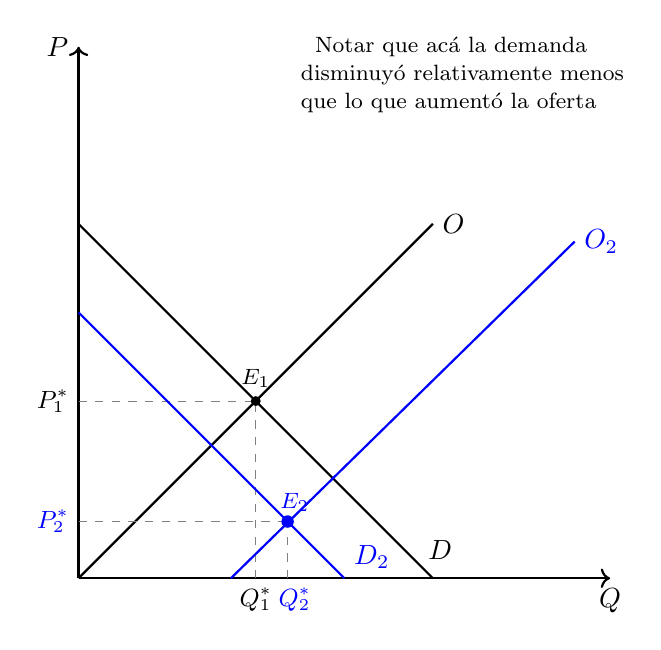
\begin{tikzpicture}[scale=0.9]
        \draw[thick,->] (0,0) -- (7.5,0) node[below] {$Q$};
        \draw[thick,->] (0,0) -- (0,7.5) node[left] {$P$};

        %Demanda
        \draw [thick] (0,5) -- (5,0);
        \node [right] at (4.8,0.4) {$D$};
        %Oferta
        \draw [thick] (0,0) -- (5,5);
        \node [right] at (5,5) {$O$};

        % Punto E
        \draw[dashed, gray] (2.5,0) -- (2.5,2.5);
        \draw[dashed, gray] (0,2.5) -- (2.5,2.5);
        \fill (2.5,2.5) circle (2pt);
        \node [above] at (2.5,2.55) {\footnotesize $E_1$};
        \node[below] at (2.5,0) {\small $Q_{1}^{*}$};
        \node[left] at (0,2.5) {\small $P_{1}^{*}$};

        % Cambios de oferta
        \draw [thick, blue] (2.15,0) -- (7,4.75);
        \node [right, blue] at (7,4.75) {$O_2$};

        % Cambios de demanda
        \draw [thick, blue] (0,3.75) -- (3.75,0);
        \node [right, blue] at (3.75,0.3) {$D_2$};

        % Nuevo equilibrio
        \draw[dashed, gray] (2.95,0) -- (2.95,0.8);
        \draw[dashed, gray] (0,0.8) -- (2.95,0.8);
        \fill[blue] (2.95,0.8) circle (2.5pt);
        \node [above, blue] at (3.05,0.8) {\footnotesize $E_2$};
        \node[below, blue] at (3.05,0) {\small $Q_{2}^{*}$};
        \node[left, blue] at (0,0.8) {\small $P_{2}^{*}$};

        \node[right] at (3.2,7.5) {\footnotesize Notar que acá la demanda };
        \node[right] at (3,7.1) {\footnotesize disminuyó relativamente menos};
        \node[right] at (3,6.7) {\footnotesize que lo que aumentó la oferta};
        
        \end{tikzpicture}
    \end{center}
    \end{figure}
\end{frame}


\begin{frame}
\frametitle{Otros ejemplos}
    \begin{enumerate}
        \item Un libro se viraliza por BookTok, pero aumenta el precio del papel de impresión
        \item Un incendio afecta la producción de yerba en Misiones, mientras el precio del té baja en los supermercados 
        \item El Estado aprueba un bono que mejora el poder de compra de jubilados, mientras se reduce un impuesto a los medicamentos
    \end{enumerate}

\end{frame}


\begin{frame}
\frametitle{Conclusiones}
    \begin{itemize}
        \item Cuando se desplace la oferta \textbf{o} la demanda (\textbf{una sola curva}), tendremos un nuevo equilibrio con un precio y una cantidad distintos.
        \item Cuando se desplacen \textbf{ambas curvas}, una de las variables del nuevo equilibrio quedará indeterminada. Es decir, dependerá de la magnitud de los cambios en la oferta y la demanda.    
    \end{itemize}
\begin{center}
\renewcommand{\arraystretch}{1.5}
\begin{adjustbox}{scale=0.8}
\begin{tabular}{|>{\columncolor{Blue!30}}c|c|c|c|c|}
\hline
\rowcolor{white}
\textbf{} & \cellcolor{red!60}\textbf{MISMA} & \cellcolor{red!60}\textbf{AUMENTO} & \cellcolor{red!60}\textbf{DESCENSO} \\
\rowcolor{white}
\textbf{} & \cellcolor{red!60}\textbf{OFERTA} & \cellcolor{red!60}\textbf{OFERTA} & \cellcolor{red!60}\textbf{OFERTA} \\
\hline
\textbf{MISMA DEMANDA} 
& \parbox[c][1.5cm][c]{2.5cm}{\centering = PRECIO \\ = CANTIDAD} 
& \parbox[c][1.5cm][c]{2.5cm}{\centering \down PRECIO \\ \up CANTIDAD}
& \parbox[c][1.5cm][c]{2.5cm}{\centering \up PRECIO \\ \down CANTIDAD} \\
\hline
\textbf{AUMENTO DEMANDA} 
& \parbox[c][1.5cm][c]{2.5cm}{\centering \up PRECIO \\ \up CANTIDAD}
& \parbox[c][1.5cm][c]{2.5cm}{\centering \question PRECIO \\ \up CANTIDAD}
& \parbox[c][1.5cm][c]{2.5cm}{\centering \up PRECIO \\ \question CANTIDAD} \\
\hline
\textbf{DESCENSO DEMANDA} 
& \parbox[c][1.5cm][c]{2.5cm}{\centering \down PRECIO \\ \down CANTIDAD}
& \parbox[c][1.5cm][c]{2.5cm}{\centering \down PRECIO \\ \question CANTIDAD}
& \parbox[c][1.5cm][c]{2.5cm}{\centering \question PRECIO \\ \down CANTIDAD} \\
\hline
\end{tabular}
\end{adjustbox}
\end{center}
\end{frame}

\end{document}
